\section{Evaluation}
Our evaluation would take the form of a case study in which we would compare different approaches to testing the {\tt function checkRows()} is Sample Code\ref{dom}, and measure how much coverage each approach can achieve.

 

checkRows() without HTML, see how far it goes
checkRows() with original HTML, see how far it goes
checkRows() with Concolic Driver, see how far it goes

Set field.children.length to 21, 

\begin{figure*}%[ht]
\centerline{\scalebox{0.38}{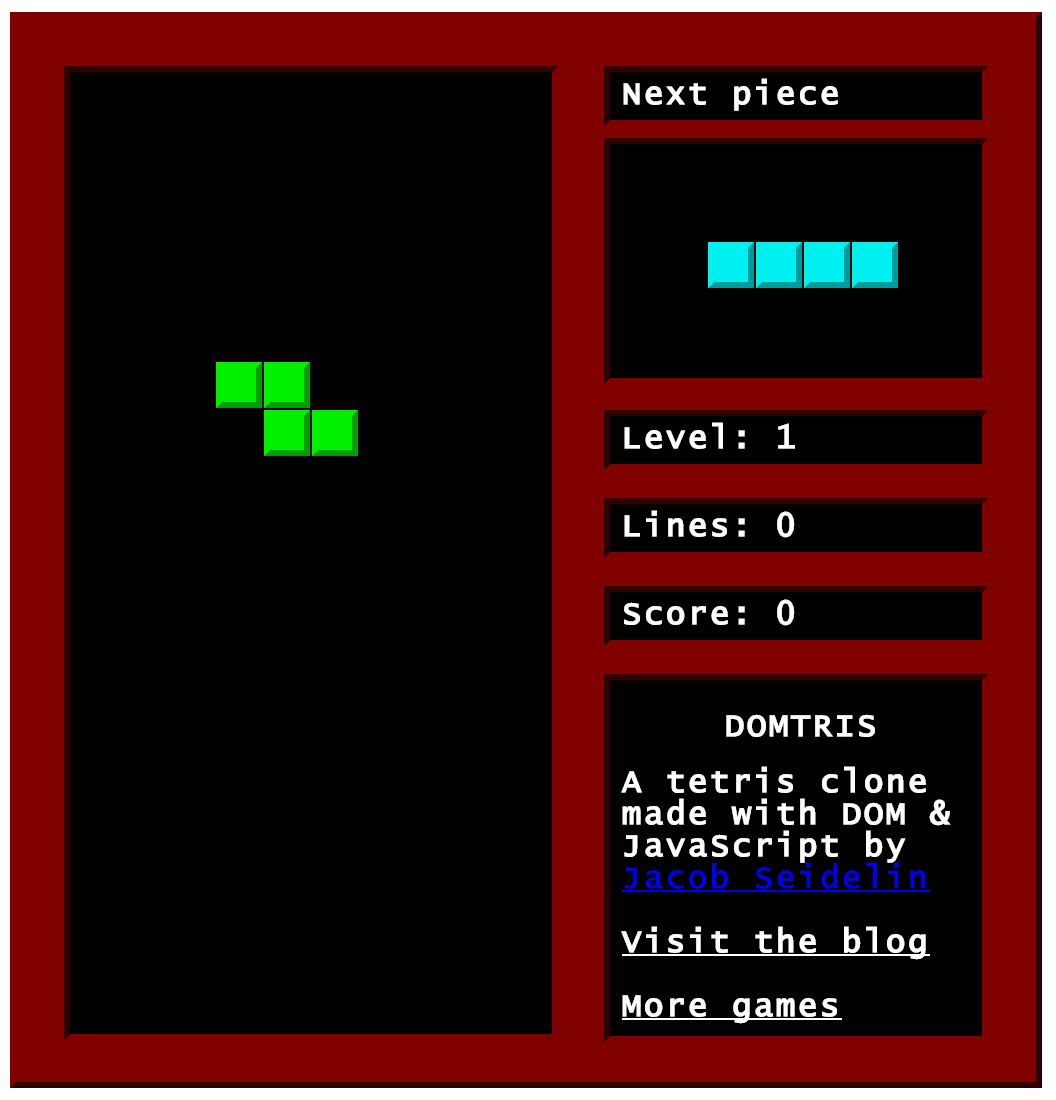
\includegraphics[natwidth=1056,natheight=1100]{domtris.png}}}
\caption[DOMtris game field]{The DOMtris game field (left) has 21 rows; thus {\tt field.children.length} should be 21.}
\label{trees}
\end{figure*}


% yahoo
% Tinysort
%  http://tinysort.sjeiti.com/
% Zen Coding
%  http://zen.sjeiti.com/
% DOMtris
%  http://www.ugrad.cs.ubc.ca/~k5r4/nbpAFZyrx5o/tracing/domtris/domtris.html
% Tudu
%  http://app.rasc.ch/tudu/welcome.action
% Knockout:
%  http://knockoutjs.com/examples/ 
% JQuery Widget: 
%  http://jqueryui.com/demos/
%  http://wijmo.com/widgets/
% Tizen
%   https://developer.tizen.org/downloads/sample-web-applications
%			mancala
